\documentclass[twocolumn]{emulateapj}
\usepackage{bm}
\usepackage{amsmath, amssymb}
\usepackage{times}
\usepackage[usenames]{xcolor}
\definecolor{mpl_red}{HTML}{D62728}
\usepackage[backref, breaklinks, plainpages=false, colorlinks=true, anchorcolor=blue!50!black, citecolor=blue!50!black, linkcolor=blue!50!black, urlcolor=mpl_red, bookmarks=false]{hyperref}
\citestyle{apj}
\usepackage[strict]{changepage}

\usepackage{natbib}


\begin{document}

% Add bracket to sectioning in the bibliography.
\renewcommand*{\backref}[1]{[#1]}

% Definition of shortcut commands.
\newcommand{\Bansal}{Karishma~Bansal}
\newcommand{\Pearlman}{\href{https:/orcid.org/0000-0002-8912-0732}{\textcolor{blue!50!black}{Aaron~B.~Pearlman}}}
\newcommand{\Majid}{\href{https:/orcid.org/0000-0002-4694-4221}{\textcolor{blue!50!black}{Walid~A.~Majid}}}
\newcommand{\Prince}{\href{https:/orcid.org/0000-0002-8850-3627}{\textcolor{blue!50!black}{Thomas~A.~Prince}}}
\newcommand{\Younes}{George~Younes}
\newcommand{\Hu}{Chin-Ping Hu}
\newcommand{\Enoto}{Teruaki~Enoto}
\newcommand{\Wharton}{Robert~S.~Wharton}
\newcommand{\Kocz}{Jonathan~Kocz}
\newcommand{\Horiuchi}{Shinji~Horiuchi}

\newcommand{\JPL}{Jet Propulsion Laboratory, California Institute of Technology, Pasadena, CA 91109, USA; \textcolor{blue}{karishma.bansal@jpl.nasa.gov}}
\newcommand{\CaltechPhysics}{Division of Physics, Mathematics, and Astronomy, California Institute of Technology, Pasadena, CA 91125, USA}
\newcommand{\GWU}{Department of Physics, The George Washington University, Washington, DC 20052, USA}
\newcommand{\APSIS}{Astronomy, Physics and Statistics Institute of Sciences (APSIS), The George Washington University, Washington, DC 20052, USA}
\newcommand{\RIKEN}{Extreme Natural Phenomena RIKEN Hakubi Research Team, RIKEN Cluster for Pioneering Research, 2-1 Hirosawa, Wako, Saitama 351-0198, Japan}
\newcommand{\Taiwan}{Department of Physics, National Changhua University of Education, Changhua 500, Taiwan}
\newcommand{\berkeley}{Department of Astronomy, University of California, Berkeley, CA 94720, USA}
\newcommand{\CSIRO}{CSIRO Astronomy and Space Science, Canberra Deep Space Communications Complex, P.O. Box 1035, Tuggeranong, ACT 2901, Australia}
\newcommand{\NDSEG}{$^{\text{9}}$~NDSEG Research Fellow.}
\newcommand{\NSF}{$^{\text{10}}$~NSF Graduate Research Fellow.}

\newcommand{\jmag}{Swift~J1818.0$-$1607}
%%%%%%%%%%%%%%%%%%%%%%%%%%%%%%%%%%%%%%%%%%%%%%%%%%%%%%%%%

\journalinfo{{\sc Submitted to The Astrophysical Journal Letters}}
\submitted{Submitted to The Astrophysical Journal}

\shorttitle{RADIO AND X-RAY OBSERVATIONS OF SWIFT J1818.0$-$1607}
\shortauthors{BANSAL ET AL.}

\title{Simultaneous Radio and X-ray observations of the Radio Magnetar Swift J1818.0$-$1607}

\author{\Bansal\altaffilmark{1}, \Pearlman\altaffilmark{2,9,10}, \Majid\altaffilmark{1,2}, \Prince\altaffilmark{2,1}, \Younes\altaffilmark{3,4}, \Hu\altaffilmark{5,6},  \Enoto\altaffilmark{5},\Wharton\altaffilmark{1}, \Kocz\altaffilmark{2,7}, and~ \Horiuchi\altaffilmark{8}}

\address{
$^{\text{1}}$~\JPL \\
$^{\text{2}}$~\CaltechPhysics \\
$^{\text{3}}$~\GWU \\
$^{\text{4}}$~\APSIS \\
$^{\text{5}}$~\RIKEN \\
$^{\text{6}}$~\Taiwan\\
$^{\text{7}}$~\berkeley\\
$^{\text{8}}$~\CSIRO}
\thanks{\NDSEG}
\thanks{\NSF}

\begin{abstract}
%%
\jmag\ is a recently discovered magnetar with a short spin period of 1.36~s 
and a magnetic field of $\sim 10^{14}$~Gauss. With an average estimated age of about 500~years, 
it is one of the youngest known isolated neutron stars with properties blurring the lines 
between high-B rotation-powered pulsars and magnetars. We have observed this source during 
multiple epochs, over a span of about six months, at high radio frequencies ($S$, $X$, and 
$Ka$ bands) using the NASA Deep Space Network. In addition, we have observed it at two epochs 
in X-ray using the Neutron Star Interior Composition Explorer (NICER) telescope. We discover 
an anti-alignment (0.40 phase cycles) in the pulse profiles of its simultaneous radio and X-ray 
observations. We discuss different models to explain this large phase offset, which is likely 
due to the X-ray emission originating at the base of the hotspots and radio from the closed 
field lines. Moreover, we report its radio properties, such as a variation in the radio flux 
densities on the time scales of hours to months; a change from steep ($\alpha < -2.2$) to flat 
spectra ($\alpha = +0.3$) in about three weeks, followed by a spectral turnover at higher 
frequencies in a span of about three months, and the varying number of radio pulse profile 
components.
\end{abstract}

\section{Introduction}
\label{sec:intro}
%%
Magnetars are neutron stars with large spin periods of $P=2-12~{\rm s}$ and extreme magnetic 
fields ($B > 10^{14}$~G). So far about 30 magnetars have been detected, and most of them 
were detected in the X-ray from either the emission of energetic bursts or pulsed emission 
\citep{kaspi2017}. Both of these emissions can be explained by the magnetar model 
\citep{duncan1992,paczynski92}. The persistent X-ray emission is expected from hotspots 
above the magnetic poles whereas, the X-ray bursts probably originate due to the large magnetic 
stress or the split and recombination of magnetic field lines. 
The luminosity of magnetar's persistent X-ray emission ranges between $10^{33}$ and 
$10^{35}~{\rm erg~s}^{-1}$ \citep{thompson2002,lyutikob2003}. Magnetars are highly variable, 
undergoing outburst episodes in conjunction with energetic short bursts, and during that time 
the number of photons increases. Based on their properties, these bursts can be divided into 
two main classes: giant flares \citep{palmer2005} and short X-ray bursts. Giant flares have an 
initial spike lasting a few milliseconds, followed by a minute-long exponentially decaying tail. 
These giant flares have a peak luminosity of $10^{44} - 10^{47}~{\rm erg~s}^{-1}$ and are very 
rare with a rough occurrence of once per decade. Short X-ray bursts are the most common bursts 
and have a duration of about a few milliseconds to seconds, and a peak luminosity in the range 
of $10^{36} - 10^{43}~{\rm erg~s}^{-1}$.%ADD REFERENCES 
 
 
Magnetars were believed to be radio-quiet until the first radio-emitting magnetar 
XTE~J1810--197 was discovered \citep{camilo2006}. In addition, four other radio 
magnetars, namely: PSR~J1745--2900 \citep{eatough2013}, PSR~J1622--4950 \citep{levin2010},
1E~1547.0--5408 \citep{camilo20071e}, and SGR~1935+2154 \citep{zhu2020}, along with a 
transitional magnetar PSR~J1119--6127 \citep{Majid+2017, pearlman2019b}, have been discovered. 
Their properties, such as the flux density, change on the timescale of seconds to months, 
and the number of components in their profile may also change. Most of these magnetars 
shut down their emission for some period and typically re-emitting a burst in X-ray. 

Swift~\jmag\ is the sixth magnetar to exhibit radio emission. 
It was discovered on March 12, 2020, when the Burst Alert Telescope was triggered by a 
soft gamma-ray-burst (GCN 28055). Subsequent follow up observations in X-ray \citep{esposito20} 
and radio \citep{champion2020} have found a spin period of $1.36$~s and 
$\dot{P} = 8.160 \pm 2 \times 10^{-11}$ s s$^{-1}$, suggesting a magnetic field of 
$3.4 \times 10^{14}$~G. Compared to typical magnetars, \jmag\ has one of the smallest 
spin periods, which is comparable to radio powered pulsars. Its profile has been found 
to be $80-100 \%$ linearly polarized across a wide observing band \citep{lower2020}. 
With an average characteristic age of $500$~yr \citep{champion2020}, it is the youngest 
known magnetars so far. 

In this article, we compare the simultaneous radio and X-ray observations of \jmag\ using 
the NASA Deep Space Network (DSN; \citealt{pearlman2019b}) and the Neutron Star Interior 
Composition Explorer (NICER) telescope, respectively. We also study how the spectral 
properties of \jmag's radio emission evolve over time. Based on these results, we draw 
comparisons of \jmag\ with other magnetars and typical radio pulsars. In Section 2.1 and 2.2, 
we describe our radio observations over six epochs and X-ray observations at two epochs. 
Then we discuss radio profile analysis in Section 3.1; radio spectral index in Section 3.2; 
our burst search in the X-ray data in Section 3.3; and X-ray profile in Section 3.4. 
We discuss these results and our implementations in Section 4 and summarize them in 
Section 5.

\section{Observations}
\label{sec:obs}
%%
\subsection{Radio}
\label{ssec:radio_obs}
%%
We carried out radio observations of \jmag\ during six epochs using different DSN radio 
telescopes (Table 1). The first two epochs (2020 March 15 and 2020 March 16) were carried 
out using DSS-35 and DSS-36, two 34\,m diameter radio telescopes in Canberra, Australia. 
Subsequent observations on 2020 March 26, 2020, April 08, and 2020 July 15 (Epoch 3, 4, and 5) 
were carried out using DSS-63, a 70\,m diameter radio telescope in Robledo, Spain. The most 
recent observation on 2020 August 10 (Epoch 6) was made using the DSS-35.

These observations were carried out in simultaneous dual frequency bands, in dual circular 
polarization mode, with center frequencies either at 2.2/8.4 GHz ($S$-band/$X$-band) or 
8.4/32 GHz ($X$-band / $Ka$-band) as noted in Table~1. The usable bandwidth was roughly 
110 MHz at $S$-band, 350 MHz at $X$-band, and 350 MHz at $Ka$-band. Data from both polarization 
channels in each frequency band were recorded in filterbank format containing channelized 
power spectral densities with the pulsar machines at each DSN complex, as described 
previously (e.g., ~\citealt{pearlman2018, pearlman2019b, Majid+2020, pearlman2020bright}). 
The time and frequency resolution for Epochs 1, 2, and 6 were roughly 512\,$\mu$s, and 
1\, MHz respectively. For epochs 3--5, the time and frequency resolution were roughly 
2.2\, ms and 0.46\, MHz respectively. Additional information for each epoch, including 
the date and the starting time of each observing session, and its duration, are 
provided in Table~1.

The data processing procedures follow similar steps to those presented in previous 
studies of pulsars and magnetars with the DSN ~(e.g.,~\citealt{Majid+2017, pearlman2018, 
pearlman2019b, pearlman2020bright}). Each data set was first corrected for bandpass slope 
across the frequency band. Subsequently, to remove low-frequency temporal variability, 
the moving average from each data value was subtracted using a 10~s window around each 
time sample. This was followed by the identification and masking of bad channels corrupted 
by radio frequency interference (RFI). The two polarization channels for each frequency 
band were then summed to form a total intensity time series. Each data set was then 
dedispersed at the nominal DM value of 706\,pc\,cm$^{\text{--3}}$ \citep{lower2020} and 
barycentered to the R.A. (J2000)$ =18^{h}18^{m}0.12^{s}$ and 
Decl. (J2000)$= -16^{\circ} 07{^\prime}52.80^{\prime\prime}$. 


\begin{deluxetable*}{ccccccc}
    \tablenum{1}
    \tabletypesize{\small}
    \tablecolumns{7}
    \tablewidth{0pt}
	\footnotesize
	\tablecaption{Radio Observations of Swift~\jmag\ with the DSN}
    \tablehead{
        \colhead{Epoch} &
        \colhead{Telescope} &
        \colhead{Obs Frequency} &
	    \colhead{Date$^{\mathrm{a}}$} &
        \colhead{Time$^{\mathrm{a}}$} &
        \colhead{Date$^{\mathrm{b}}$} &
        \colhead{Duration} \\
        \colhead{} &
        \colhead{} &
        \colhead{(GHz)} &
		\colhead{} &
        \colhead{(hh:mm:ss)} &
        \colhead{(MJD)} &
		\colhead{(hr)}
        }
        \startdata
	1 & DSS-35 & 8.4, 32  &2020 Mar 15 & 21:14:60 & 58923.88541 & 0.7 \\
	2 & DSS-36 & 2.2, 8.4 & 2020 Mar 16 & 23:00:01 & 58924.95833 & 1.9 \\
	3 & DSS-63 & 2.2, 8.4 & 2020 Mar 26 & 08:29:60 & 58934.35417 & 2.1 \\
	4 & DSS-63 & 2.2, 8.4 & 2020 Apr 08 & 07:37:54 &  58947.31799 & 1.9 \\
	5 & DSS-63 & 2.2, 8.4 & 2020 Jul 15 & 19:46:38 &  59045.82405 & 2.1 \\
	6 & DSS-35 & 8.4, 32  & 2020 Aug 10  & 10:30:00 & 59071.43750 & 1.6 \\
        \enddata
        \tablecomments{Parameters for the six dual-frequency observations.\\
                $^{\mathrm{a}}$ Start date and time of the observation (UTC).\\
                $^{\mathrm{b}}$ Start day of the observation (UTC).}
        \label{Table:RadioObservations}
\end{deluxetable*}

%% The above MJDs have not been corrrected for 1 second delay

%%%%%%%%%%%%%%%%%%%%%%%%%%%%%%%%%%%%%%%%%%%%%%%%%%%%%%%%%%%%%%    

\subsection{X-ray}
\label{ssec:xray_obs}
%%
X-ray observations of \jmag\ were carried out using the \textit{NICER} X-ray Timing 
Instrument (XTI) \citep{gendreau2016}, operating on the International Space Station. 
It operates in the soft X-ray energy range of $0.2-12$~keV with an effective area of 
$1900~{\rm cm}^{2}$ at 1.5~keV. It has absolute timing precision of $< 300$~ns. 
We observed \jmag\ on March 26, 2020 (Id: 3556011101), and April 04, 2020 (Id: 3556011801), 
for a duration of 2515 and 2890 seconds, respectively. These observations were part of 
the larger NICER program to monitor this source \citep{hu2020}. 

Initial data cleaning and reduction was carried using the Heasoft version 6.28 
\citep{heasoft14}. We filtered out the times with a high background count, near the 
South Atlantic Anomaly (SAA), when the angular separation was more than $0.015^{\circ}$, 
and when the elevation angle was less than $30^{\circ}$ above the limb of the Earth or 
less than $40^{\circ}$ above the bright Earth limb. The events times were converted to 
barycenter time using the same coordinates as the radio observations (section 2.1) and 
the JPL DE405 solar system ephemeris.%\abp{[Specify that these are J2000 coordinates.]}
 
\section{Results}
\label{sec:results}
%
\begin{figure*}[b]
    \begin{tabular}[b]{@{}p{0.24\textwidth}@{}}
    \centering\small (a) 26 March
	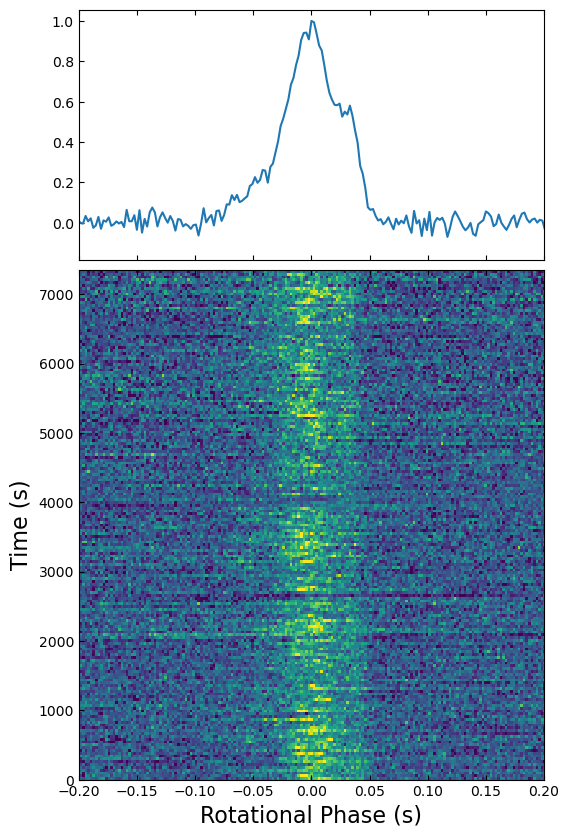
\includegraphics[width=\linewidth]{plots/s-band_Mar26.png}
    \end{tabular}
    \begin{tabular}[b]{@{}p{0.24\textwidth}@{}}
    \centering\small (b) 08 April
	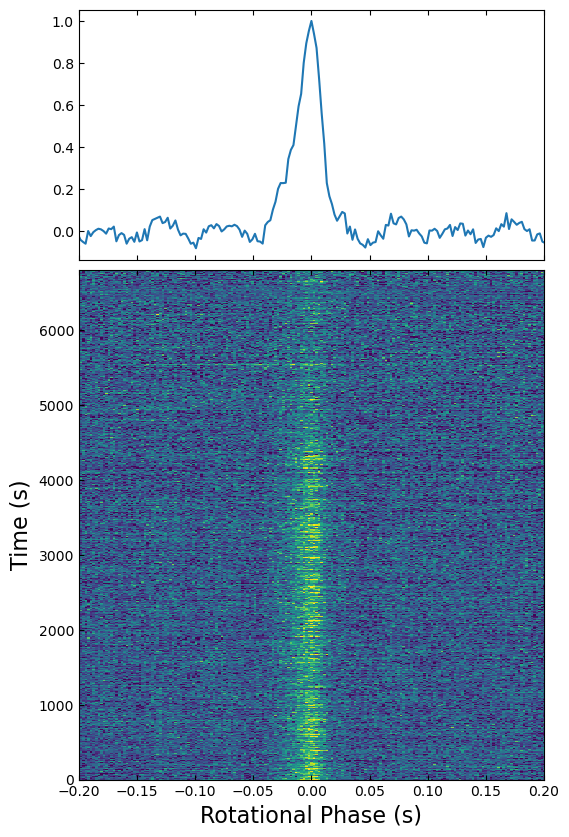
\includegraphics[width=\linewidth]{plots/s-band_Apr08.png}
    \end{tabular}
    \begin{tabular}[b]{@{}p{0.24\textwidth}@{}}
    \centering\small (c) 15 July
	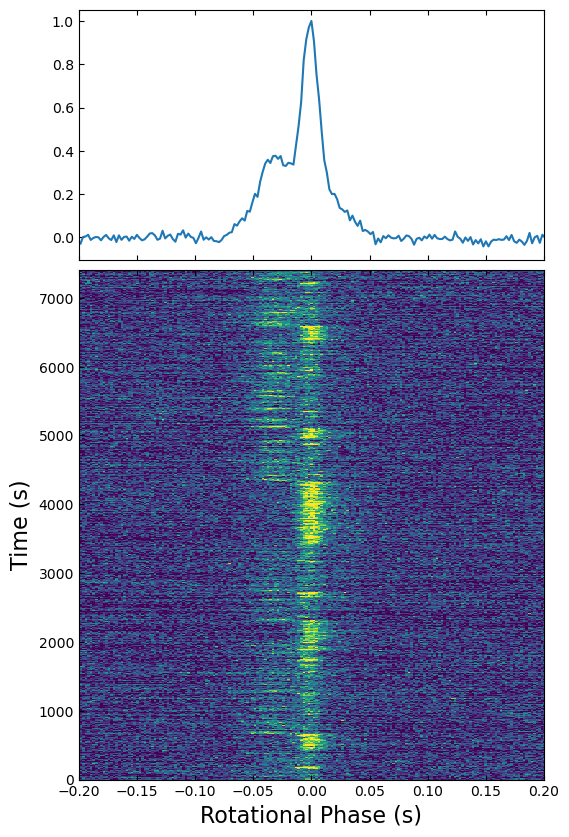
\includegraphics[width=\linewidth]{plots/s-band_Jul15.png}
    \end{tabular}
    \setlength\arrayrulewidth{2pt}
    \begin{tabular}[b]{|@{}p{0.24\textwidth}@{}}
    \centering\small (d) 10 August
	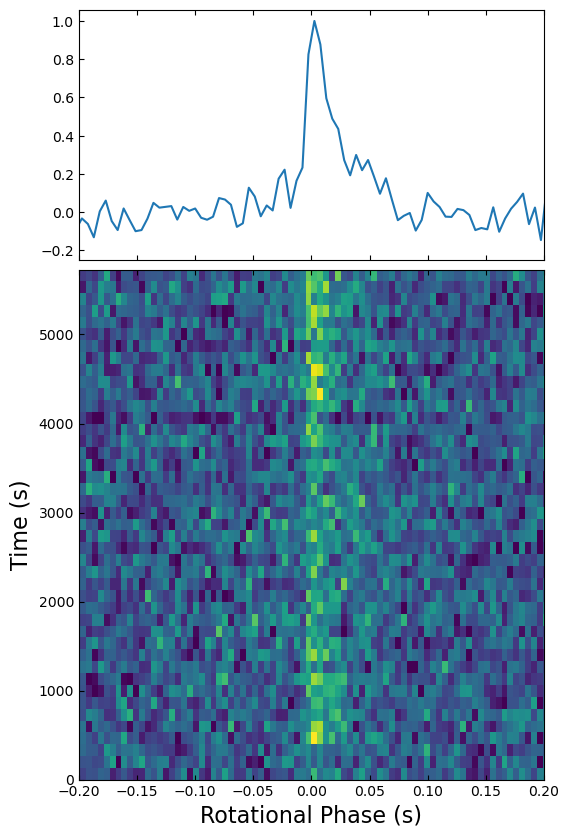
\includegraphics[width=\linewidth]{plots/ka-band_Aug10.png}
    \end{tabular}
    \quad
    
    \begin{tabular}[b]{@{}p{0.24\textwidth}@{}}
    {}
    \end{tabular}
    \begin{tabular}[b]{@{}p{0.24\textwidth}@{}}
    \centering
	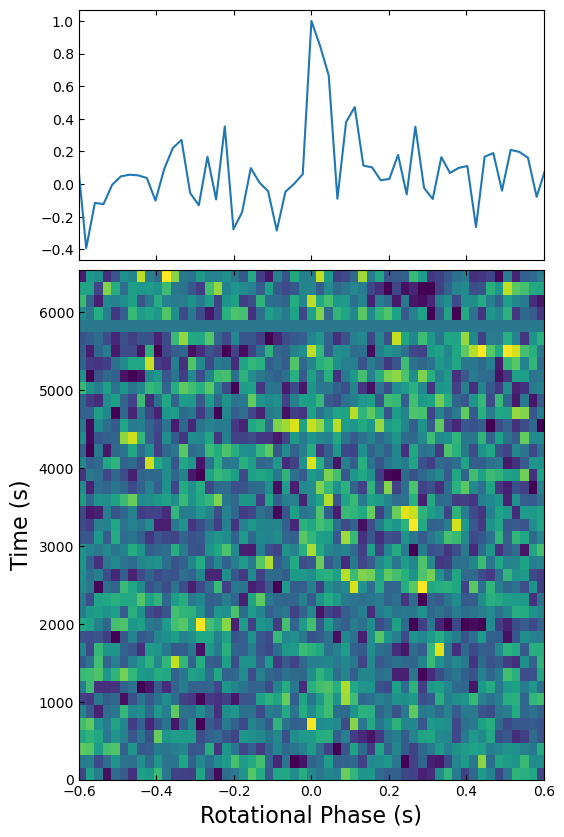
\includegraphics[width=\linewidth]{plots/x-band_Apr08.png}
    \end{tabular}
    \begin{tabular}[b]{@{}p{0.24\textwidth}@{}}
    \centering
	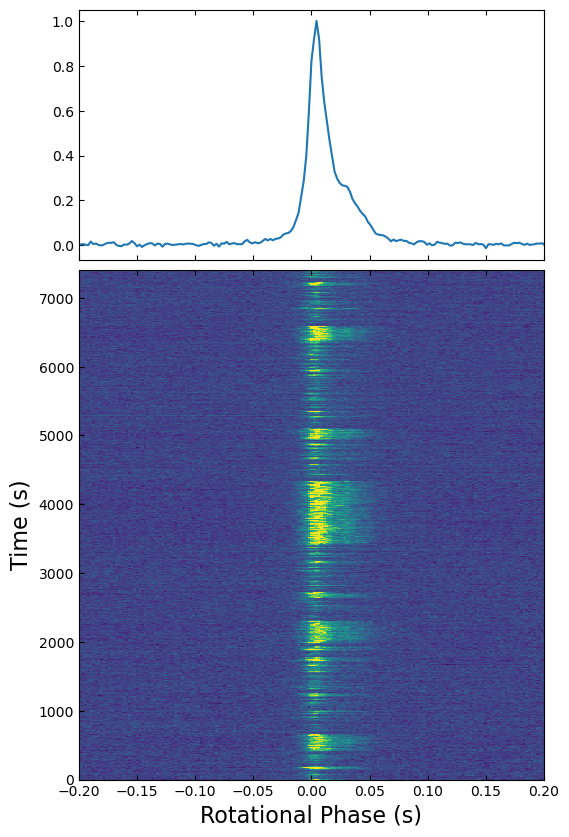
\includegraphics[width=\linewidth]{plots/x-band_Jul15.png}
    \end{tabular}
    \begin{tabular}[b]{@{}p{0.24\textwidth}@{}}
    \centering
	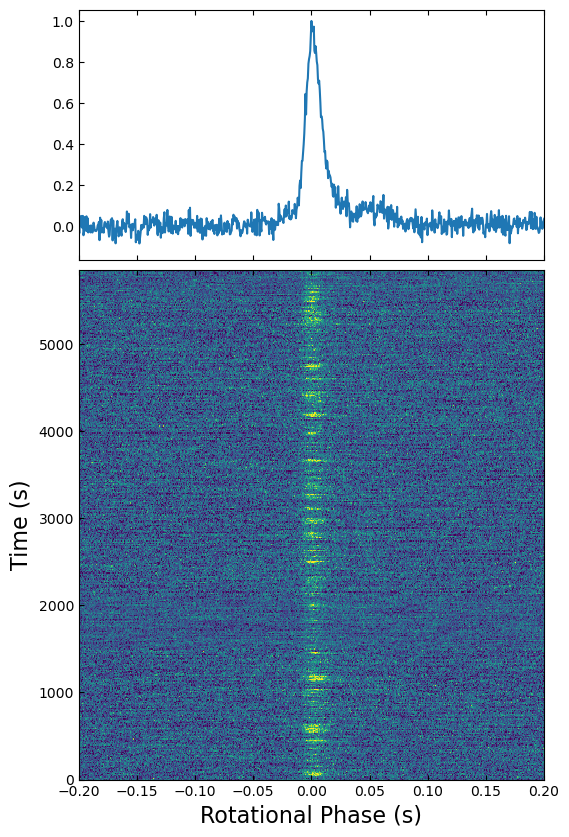
\includegraphics[width=\linewidth]{plots/x-band_Aug10.png}
    \end{tabular}
    \quad 

    \caption{Folded radio profiles from the four observations with 
             detections.  The top row shows \jmag\ at 2.4~GHz (a-c) 
             and 32~GHz (d), and the bottom row shows 8.4~GHz.  Note 
             that \jmag\ shows profile evolution on both long (days-months) 
             and short (seconds-minutes) timescales.  The short timescale 
             changes on 15~Jully are the result of mode-switching 
             (Figure~\ref{fig:modes}) shows this in more detail.
            }
	\label{fig:radio_profs}
\end{figure*}


\begin{figure*}[b]
	\centering
	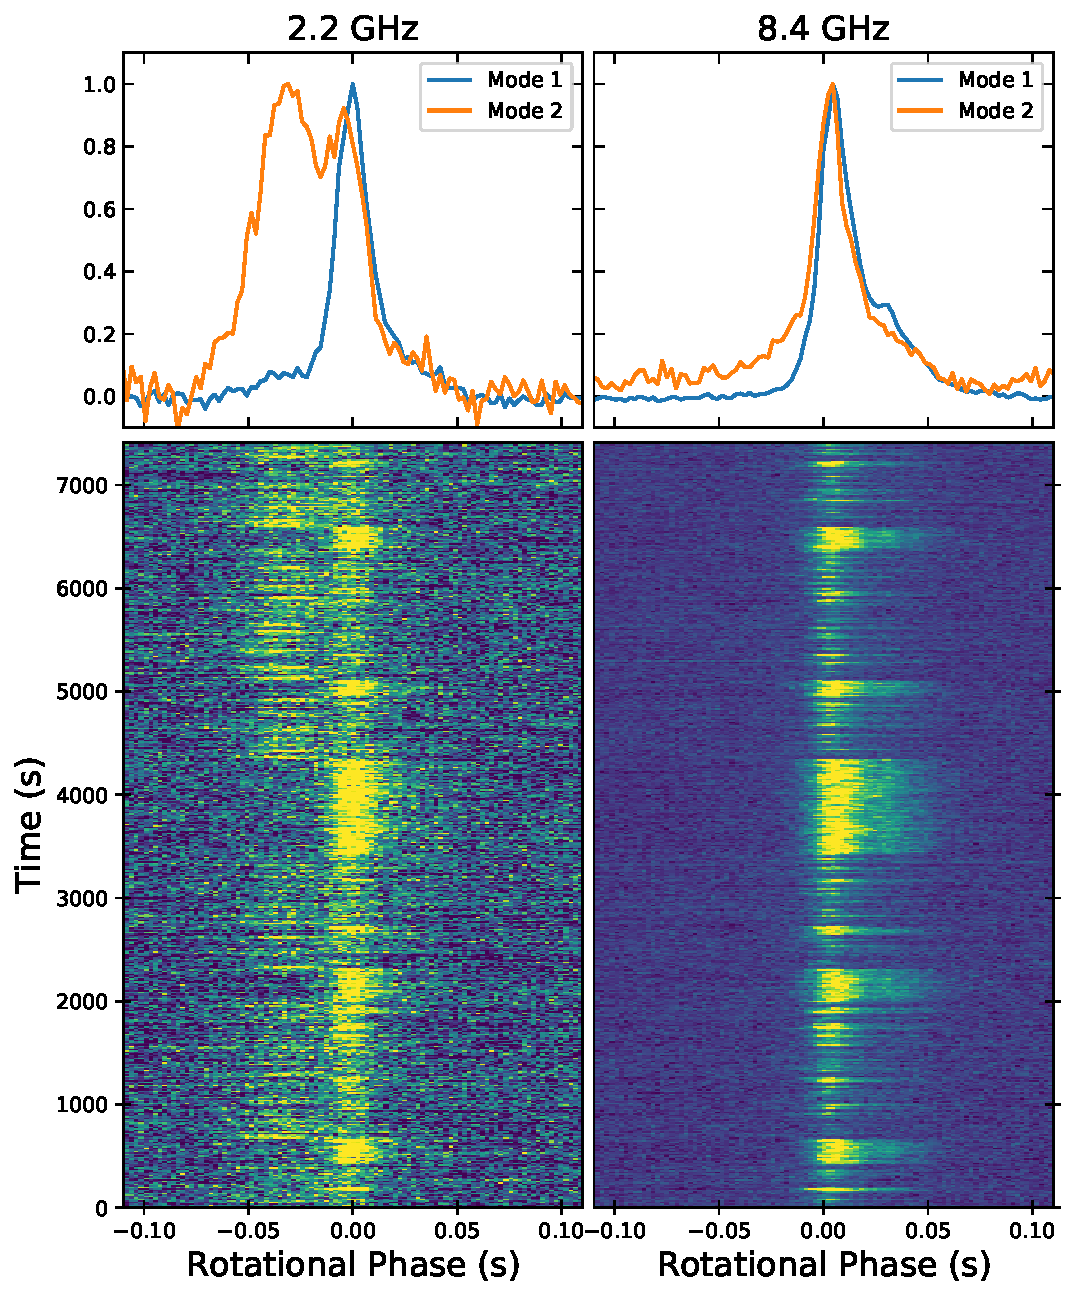
\includegraphics[width=0.75\linewidth]{plots/sx-mode.pdf}
	\caption{Mode switching in \jmag\ at 2.2 and 8.4~GHz on 15 July 2020.  
             Each panel shows the changing pulse shape at both frequencies 
             over the course of the observation.  Mode~1 corresponds to 
             the bright mode at 8.4~GHz and Mode~2 the fainter mode.  The 
             integrated pulse profiles from just the rotations in Mode 1 
             and Mode 2 are show in the top panels.  In both cases Mode 1 
             is much brighter, but the profiles have been normalized so that 
             the peak of each is the same.}
	\label{fig:modes}
\end{figure*}


\begin{figure*}[b]
	\centering
	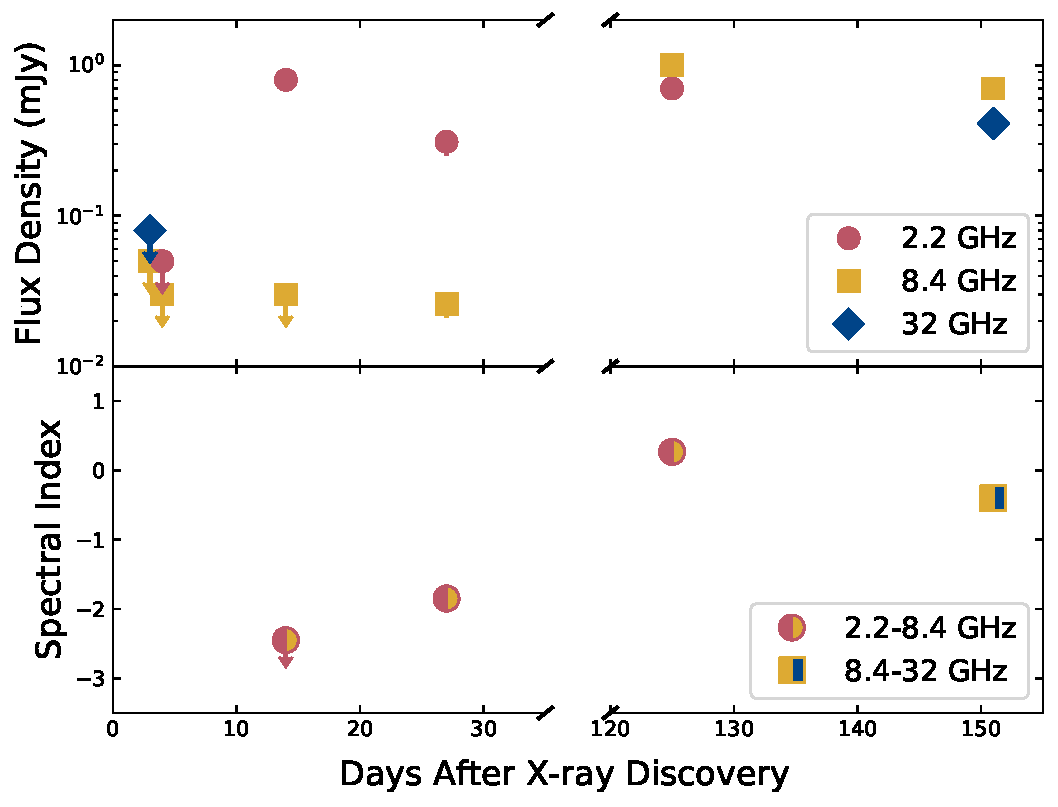
\includegraphics[width=0.75\linewidth]{plots/J1818_flux_spec.pdf}
	\caption{\emph{Top:} Period-averaged flux density measurements of 
             \jmag\ from dual band 2.2/8.4~GHz and 8.4/32~GHz observations. 
             Non-detections show the $7\sigma$ upper limits.  \emph{Bottom:} 
             Spectral indices derived from the dual-band observations.}
	\label{fig:flux_spec}
\end{figure*}




\begin{deluxetable*}{lccccc}
    \tablenum{2}
    \tabletypesize{\small}
    \tablecolumns{6}
    \tablewidth{0pt}
	\footnotesize
	\tablecaption{Rotational Period and Flux Density Measurement of Swift~\jmag}
    \tablehead{
        \colhead{Epoch} &
        \colhead{F0} &
        \colhead{S(2.2~GHz)} &
        \colhead{S(8.4~GHz)} &
        \colhead{S(32~GHz)} &
        \colhead{Spectral Index} \\
        \colhead{} &
        \colhead{(Hz)} &
	\colhead{(mJy)} &
        \colhead{(mJy)} &
         \colhead{(mJy)} &
	\colhead{}\\
        }
        \startdata
    1 & $-$           & $-$       & $<0.05$   & $<0.08$  &  $-$    \\
	2 & $-$           & $<0.05$   & $<0.03$   & $-$      &  $-$    \\
	3 & 0.7333684(2)  & 0.80(2)   & $<0.03$   & $-$      & $<-2.2$ \\
	4 & 0.73335175(6) & 0.31(6)   & 0.026(5)  & $-$      & $-1.9(2)$ \\
	5 & 0.7331469(2)  & 0.70(1)   & 1.00(2)   & $-$      & $+0.3(2)$ \\
	6 & 0.73309715(8) & $-$       & 0.7(1)    &  0.41(8) & $-0.4(2)$ \\
        \enddata
        \tablecomments{Measured period averaged flux density of \jmag\ 
                       at each observing epoch.  When no pulsations were 
                       detected we report a $7\sigma$ upper limit.  Spectral 
                       indices are measured between the two frequencies 
                       observed.  In the event that there is no detection 
                       at one of the frequencies we report a $x\sigma$ limit.}
        \label{tab:flux}
\end{deluxetable*}

\subsection{Radio Profiles}
\label{ssec:radio_profiles}
%%
We searched all datasets for evidence of pulsed emission near the 
spin period of the pulsar after dedispersing the data. No pulsed emission 
was detected on either 15 March (8.4/32~GHz) with DSS-35 or 
16 March (2.2/8.4~GHz) with DSS-36.  On 26~March, we observed with the 
70-m dish DSS-63 at 2.2/8.4~GHz and detected pulsed emission at 2.2~GHz 
but not 8.4~GHz.  On 08~April, we again detect \jmag\ at 2.2~GHz and 
make a marginal detection at 8.4~GHz. By 15~July, the magnetar is much 
brighter and very strong detections are made at both 2.2 and 8.4~GHz.  
With the magnetar apparently getting brighter at higher frequencies, we 
switched back to observing with the 34-m DSS-35 at 8.4 and 32~GHz on 
10~August and made detections at both frequencies.  The integrated and 
time-resolved pulse profiles all the detections are shown in 
Figure~\ref{fig:radio_profs}.

Like other radio-emitting magnetars, \jmag\ shows significant pulse 
profile evolution over time.  At 2.2~GHz, the average pulse shape 
starts out fairly wide on 26 March with perhaps a trailing shoulder, 
then narrows by 08~April, before gaining a new leading component 
on 15 July.  Similar pulse shape changes around the same time were 
also seen with the high cadence multi-frequency campaign of 
\citet{champion2020}, the 2.25/8.40~GHz observations of 
\citet{huang2021}, and the wideband $0.7-4$~GHz observations of 
\citet{lower2021}.   

In addition to long-term evolution, we also see short-term variations 
in the form of mode switching.  This is most prominent in the 15~July 
observations at 2.2/8.4~GHz.  Figure~\ref{fig:modes} shows a side by side 
comparison of the pulse shapes at 2.2 and 8.4~GHz over the course of the 
observation.  The dispersive delay has been removed, so the zero point 
of the phase is the same at each frequency.  The profiles at both 
frequencies seem to switch between two modes.  At 8.4~GHz, one mode 
is much brighter than the other, though the profile shapes are similar. 
At 2.2~GHz, the mode-switching occurs at exactly the same time as at 
8.4~GHz.  However, the pulse shape seems to change significantly from 
a single to double component profile.  \citet{huang2021} also report 
simultaneous mode switching at 2.25/8.40~GHz around the same time 
as our observations and moding at other frequencies has also been 
reported by others \citep{lower2021, rajwade2022}. 


\subsection{Radio Flux Density and Spectral Index}
\label{ssec:spec}
%%
By simultaneously observing at two different frequency bands, 
our observations allow for simple spectral index measuremnts 
of \jmag\ in the months after its discovery.  
The period-averaged flux density measurements for all detections 
are given in Table~\ref{tab:flux}.  For non-detections, we set 
$7\sigma$ upper limits assuming a detection limit of 

\begin{equation}
  S_{\rm min} = \frac{({\rm S/N})_{\rm min} \, T_{\rm sys}}
                       {G \sqrt{n_{\rm p} \Delta \nu T_{\rm obs}}} 
                \sqrt{\frac{\delta}{1-\delta}}
\label{eqn:snr}
\end{equation} 

where $\rm (S/N)_{\rm min} = 7$ is our detection threshold, 
$T_{\rm sys}$ and $G$ are the system temperature and gain of 
the telescope, $n_{\rm p} = 2$ is the number of polarizations 
summed, $\delta \nu$ is the frequency bandwidth, $T_{\rm obs}$ 
is the observing time, and $\delta = W/P = 0.1$ is the assumed 
duty cycle of the pulsar.  For epochs in which detections are 
made at both frequencies, we can measure a spectral index 
assuming the flux density follows a power-law form 
of $S_{\rm \nu} \propto \nu^\alpha$.  For epochs with one 
detection and one limit, we set a $7\sigma$ limit.  The 
spectral indices and limits are given in Table~\ref{tab:flux}.

Figure~\ref{fig:flux_spec} shows the spectral index evolution 
out to about 150~days after the initial X-ray discovery 
on 12~March~2020 \citep{esposito20}.  After two non-detections 
on 15 and 16~March, our first detection of \jmag\ on 
26~March had a very steep 2.4-8.4~GHz spectral index of 
$\alpha_{2-8} < -2.2$.  By 08~April, the spectral had flattened 
to $\alpha_{2-8} = -1.9 \pm 0.2$, which is more in line with 
typical radio pulsar spectral indices \citep[e.g.,][]{maron2000}. 
The spectral continued to flatten so that by 15~July the spectral 
index was actually slightly inverted at $\alpha_{2-8} = +0.3 \pm 0.2$. 
Interestingly, one component in the 2.4~GHz profile on 15~July 
(Figure~\ref{fig:radio_profs}c) has a steep spectrum and does 
not show up at 8.4~GHz, while the other is inverted and gets 
brighter at 8.4~GHz.  This is consistent with the so-called 
magnetar and pulsar modes seen by \citet{lower2021}.  Finally, 
on 10~August we measure the 8.4-32~GHz spectral index to be 
$\alpha_{8-32} = -0.4\pm 0.2$.  The general trend of spectral 
flattening is consistent with the initial detections of 
\citet{champion2020} and corroborate the much longer term 
2.25/8.60~GHz measurements of \citet{huang2021}. 






\begin{figure*}[b]
	\centering
	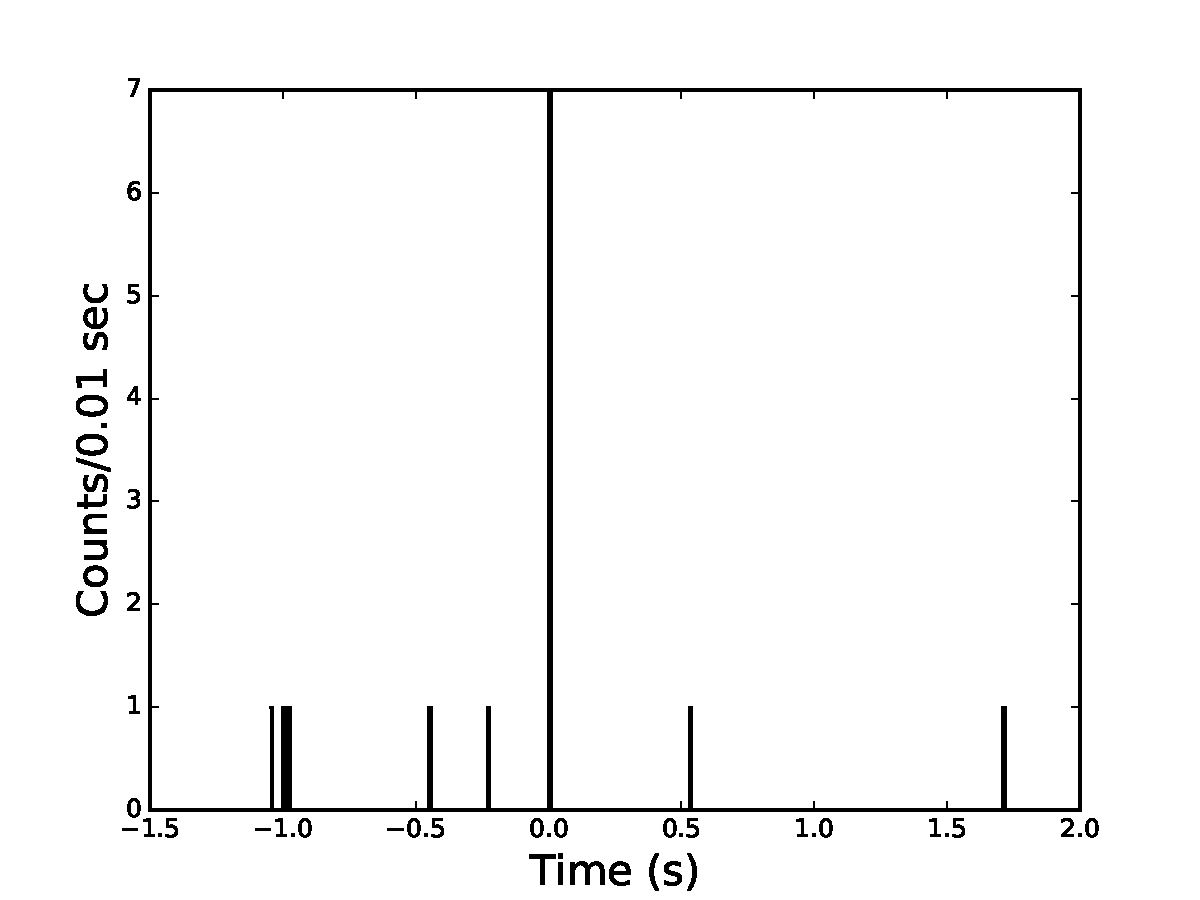
\includegraphics[trim=0cm 0cm 0cm 0cm, clip=false, scale=0.55, angle=0]{plots/J1818_burst_light_curve.pdf}
	\caption{Light curve of a short X-ray burst in \jmag\, in the energy 
             range 0.3-10 keV (Section 3.3). The number of photons in this burst 
             are 5 and its width is 0.0015 s. It was observed using the NICER 
             telescope with observation Id:3556011801.} 
	\label{fig:xray_burst}
\end{figure*}

\subsection{X-ray Bursts}
\label{ssec:xray_bursts}
%%
We carried out a search for X-ray bursts in both X-ray observations (see Section 2.2) 
using unbinned event times. We employ the technique of Bayesian blocks \citep{scargle12} 
which obtains optimal bins for a given dataset. This is a robust technique as it does 
not depend on the sampling or bin size of a dataset and can detect local structures 
in highly variable datasets. The datasets are first divided into optimum segments (blocks) 
such that there is no overlap between them and all model parameters, such as event rate, 
are constant within each block. The boundaries where a statistical model undergoes an 
abrupt change are called edges. These edges are used to form optimal histograms which 
help in identifying local structures \citep{lin13}. This prior distribution of blocks 
($ncp_{prior}$) is obtained using Equation 21 in \cite{scargle12}, which depends on 
the number of events ($N$) and the false probability ($p0$). In this paper, we use 
an inbuilt Bayesian  Block function from AstroPy, with $p0 = 0.05$.

In our first X-ray observation of \jmag\, the edges overlap with the good time intervals 
(GTIs) suggesting that there are no bursts during this observation. However, for the 
second X-ray observation, we note that the number of edges is more than the number GTIs. 
Upon a closer investigation, we find a block at MJD 58947.2201 with a sudden increase 
in the count rate in a short duration, suggesting a soft x-ray burst. The number of 
photons in this burst is 5 and its duration is 0.0013 s. Its width has been obtained 
from the size of the representative Bayesian block. The mean count rate for this 
observation is 1.2 counts s$^{-1}$, which has been obtained from the spectral fitting 
in the energy range of 0.3--10 keV \citep{hu2020}. For the duration of this burst, the 
mean count is 0.002. Assuming a Poisson distribution, we obtain the false alarm 
probability of this burst to be 2.7e-16. We have plotted the light curve of this 
burst in Figure~\ref{fig:xray_burst}. However, due to the low number of counts 
in this burst, we were unable to fit its spectrum.

%  We estimate the signal-to-noise ratio (SNR) ($N/\sqrt(N+B)$) of this burst to be 2.5 $\sigma$ using the estimated background rate (b). From these SNRs, we conclude that this burst is statistically insignificant.%We find the total significance of this burst to be $2.5\sigma$, % <<THE ESTIMATE OF SIGNIFICANCE FOR INDIVIDUAL SPECTRA IS EVEN LOWER SO I WONDER IF WE SHOULD INCLUDE THAT>> %\textit{nicer\_bkg\_estimator}\footnote{\url{https://heasarc.gsfc.nasa.gov/docs/nicer/tools/nicer_bkg_e st_tools.html}}. It is a space weather based method (Gendreau et al., in prep) which obtains the background spectra of an observation based on the time-dependent particle background, optical loading from the Sun, and the diffuse sky background. 

 
%%  Obtain the significance of burst in each energy range
%The top panel shows burst in the .. ..  We obtain various light curves with binsizes ranging from 0.001 till 1 seconds (Figure ). At both epochs we obtain one bursts which persists across these binsizes. 


\subsection{X-ray Profiles}
\label{ssec:xray_prof}
%% 
We obtain absolute X-ray phases for both epochs using PINT built-in functions 
\citep{Luo2019}, and the ephemeris obtained from contemporaneous radio analysis. 
We fold the X-ray data and obtain average X-ray profiles, one for each epoch. 
This is done using NICERSoft program \footnote{https://github.com/paulray/NICERsoft}, 
which uses the absolute phases, and filters out events with energies less than 2 keV 
and greater than 6 keV to select the most sensitive band of NICER telescope. 
In Figure~\ref{fig:xray_radio}, we plot the average X-ray pulse profiles (black) 
as well as the phaseogram for both epochs. Note that for Epoch 4 
(Figure~\ref{fig:xray_radio}b), GTIs before and including the tentative 
X-ray burst have been excluded. The pulsed X-ray emission is consistent within the 
observation duration for each epoch, with no indication of any glitch. The RMS pulsed 
fraction \citep{an2015} for Epoch 3 and Epoch 4 are $0.31 \pm 0.02$ and $0.36 \pm 0.03$, 
respectively. This increase in the pulsed fraction is consistent with those reported 
in \cite{hu2020}. We note that the X-ray pulse profile in the second observation 
has more structure as compared to that of the first one.
%(MAYBE COMPARE THE FITTING PARAMETERS).

To investigate if there is any phase correlation between our simultaneous observations 
in radio and X-ray, we overlay the $S$-band average profiles (red) on X-ray profiles 
for both epochs. The location of the pulse peak in the X-ray profiles was obtained 
by fitting a sinusoidal function (blue). At both epochs, the peak of the radio pulse 
profile at $S$-band leads the X-ray pulse profile with a phase offset (in phase cycles) 
of $0.40 \pm 0.03 $ and $0.33 \pm 0.03$, respectively. This offset implies that the 
peaks of radio and X-ray are almost misaligned with the radio occurring at X-ray pulse 
minimum. We validated this procedure by comparing the radio and X-ray profiles of the 
Crab pulsar. We confirmed that the peak of its radio profile at the S-band aligns with 
the peak of its X-ray profile, as expected \citep{hankins2007}. We analyzed the recent 
NICER observation of \jmag\ in February 2021, to further test this phase misalignment, 
but no pulsed emission was detected in the X-ray.


\begin{figure*}[b]
	\centering
	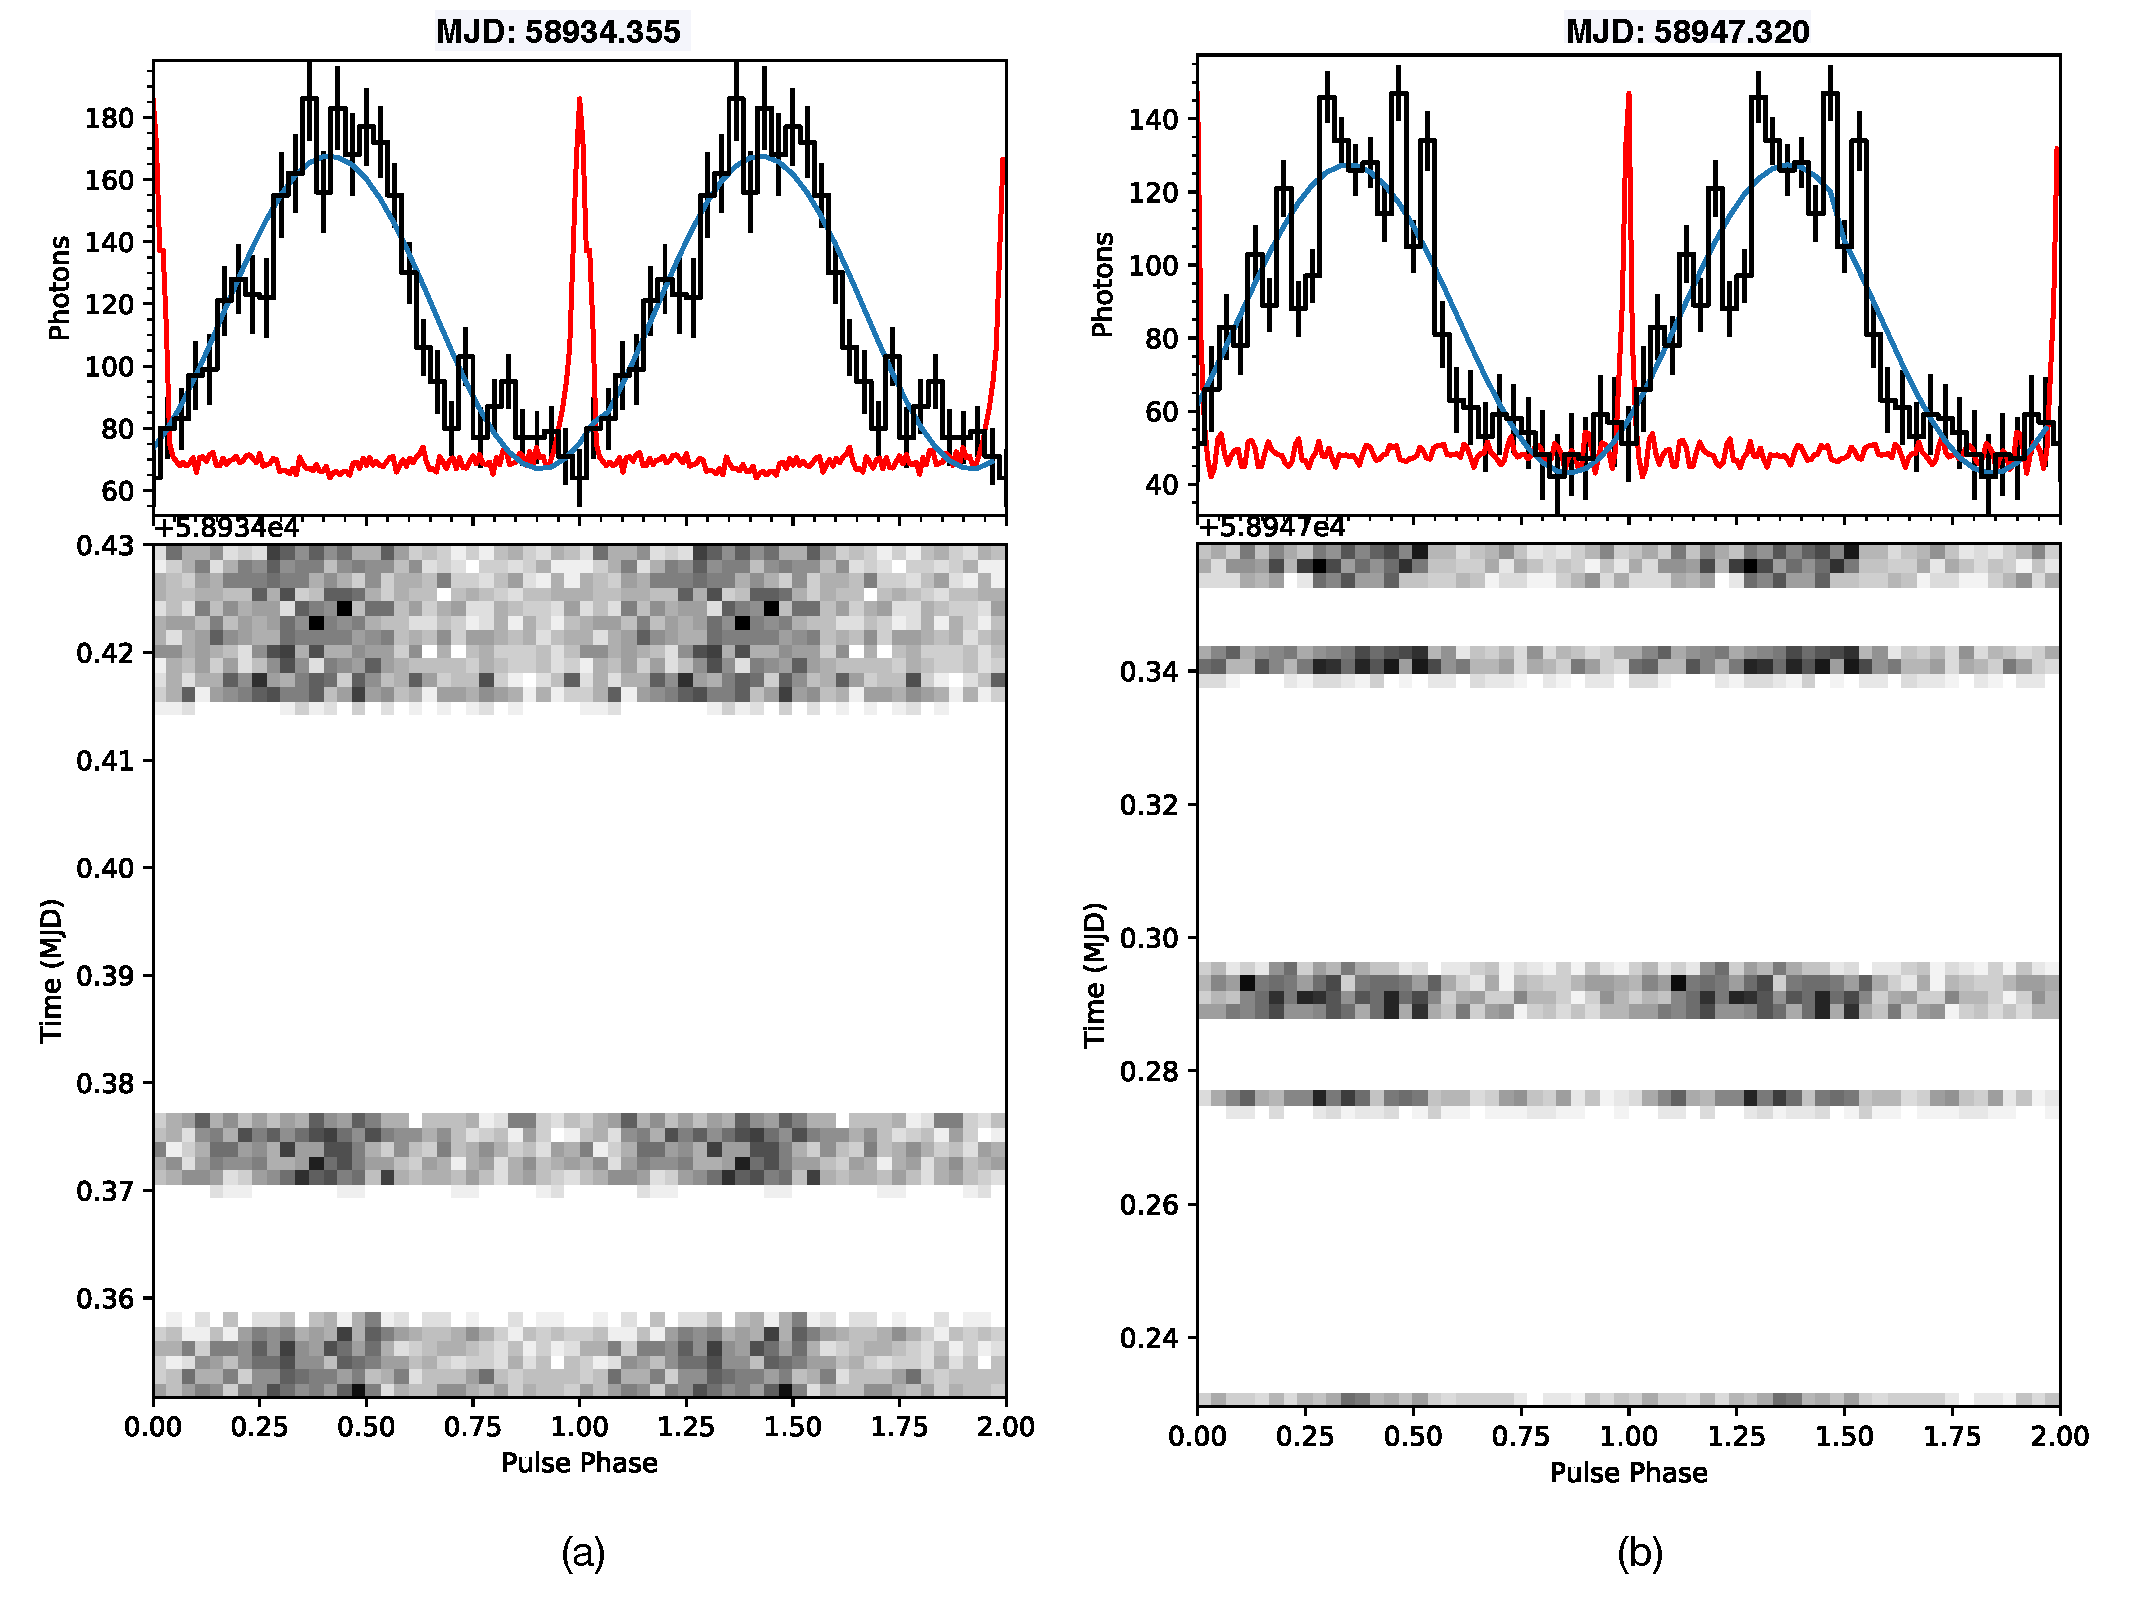
\includegraphics[trim=0cm 0cm 0cm 0cm, clip=false, scale=0.4, angle=0]{plots/average_phaseogram.pdf}
	\caption{ Integrated pulse profiles and phaseogram of \jmag\ at X-ray (black) 
              during MJD 58934.35 (panel 1) and 58947.33 (panel 2). We fit each X-ray 
              profile using a sinusoidal function (blue) and overlay the corresponding 
              average pulse profile at $S$-band (red). The phase offset between radio 
              and X-ray profile are $0.40 \pm 0.03 $ (a) and $0.33 \pm 0.03$ (b).}
              %\abp{Remove white space at the start, in the bottom panels. Also, don't use 
              % scientific notation for the MJD times along the y-axis, and use fewer bins 
              % in the X-ray pulse profile.]} 
    \label{fig:xray_radio}
\end{figure*}

%%%%\section{Discussion}
%%%%\label{sec:discussion}
%%%%%%
%%%%\subsection{Comparison with Magnetars}
%%%%\label{ssec:compare_mag}
%%%%%%
%%%%We search for X-ray bursts in our NICER observations of \jmag\ and detect one X-ray 
%%%%burst. In a recent study, \cite{hu2020} reported additional 18 X-ray bursts from 
%%%%this source, detected using the NICER telescope. We also report the averaged X-ray 
%%%%pulsed emission from \jmag\ from two epochs in Figure~\ref{fig:xray_radio}. Thus, 
%%%%\jmag\ shows both persistent X-ray emission as well as a prolific number of X-ray bursts, 
%%%%a hallmark of magnetars.
%%%%
%%%%%Using the above estimated $\dot{\nu}$ value (see Section 3.1), we obtain an average 
%%%%%period derivative, $\dot{P}$ of $4.34 \times 10^{-11}$ s s$^{-1}$ 
%%%%%(Figure~\ref{fig:spindown}). 
%%%%%We estimate the dipolar B-field strength at the equator ($\propto \sqrt(P \dot{P})$) 
%%%%%to be $2.5 \times 10^{14}$ Gauss and the characteristic age ($\frac{P}{2\dot{P}}$) 
%%%%%is about 500 years. These overall characteristics compare well with other magnetars. 
%%%%%Our measurement of $\dot{P}$ as compared to recent studies \citep{esposito20, lower2020} 
%%%%%is about two times smaller, and matches with those by \cite{champion2020, hu2020}, and 
%%%%%\cite{huang2021}. Note that all the estimates of $\dot{F}$ are unreliable due to the 
%%%%%strong timing noise in this source; thus, the true age significantly differs from the 
%%%%%spin-down age. This is not surprising as $\dot{F}$ is often observed to vary in magnetars, 
%%%%%especially during periods of bursting activity. Moreover, the estimated characteristic age 
%%%%%is not a good indicator of its age as it assumes magnetic dipole radiation, which is likely 
%%%%%not the case for magnetars. Perhaps an estimate of proper motion will provide a more robust 
%%%%%estimate of age if an association with a supernova remnant is found 
%%%%%\citep{blumer2020,lower2020, Gaensler2000}. Moreover, kinetically derived age is 
%%%%%independent of an emission mechanism.  
%%%%
%%%%From our radio analysis, we see a large variation in the flux density of \jmag\ over 
%%%%various timescales, ranging from hours to months (Figure~\ref{fig:radio_profs}). 
%%%%At $X$-band, it goes from a null detection at the first few epochs to a $5\sigma$ 
%%%%detection from Epoch 4 
%%%%onward. The flux density of \jmag\ at $X$-band increases by a factor of 40 between 
%%%%Epochs 4 and 5. Similarly, there is a null detection at $Ka$-band in Epoch 1, with 
%%%%a flux density of 0.41 mJy in Epoch 6. Moreover, during Epoch 5, there is a change 
%%%%in the flux density on the timescale of hours during our observation at both $S$ 
%%%%and $X$-band (Figure~\ref{fig:radio_profs}c). In contrast to our null detection 
%%%%in the first few epochs, \cite{champion2020} detect pulse emission in Epoch 1 at 
%%%%1.5 and 2.5 GHz, and Epoch 2 
%%%%at 1.5 GHz. As the observing frequencies in \cite{champion2020} are lower than our 
%%%%corresponding frequencies (Table 1), our non-detections are due to the steep spectrum 
%%%%of \jmag\ at these epochs. Similarly, there is a change in the spectral index of \jmag 
%%%%between $S$-band and $X$-band as it goes from a steep spectrum of $< -2.2$ at Epoch 3 
%%%%to a flat spectrum of $+0.3$ at Epoch 5, over a period of about three months.  
%%%%A similar variation in the spectral index ($-0.97$) has been reported in a recent 
%%%%observation of \jmag\ \citep{Liu2020}. In Epoch 6, we see a spectral turnover with 
%%%%an index of $-0.4$ between 8.4 GHz and 32 GHz, consistent with a recent estimate 
%%%%of $-1.4$ between 86 and 154 GHz \citep{Torne2020}. 
%%%%
%%%%
%%%%The above characteristics of \jmag\ are analogous to other radio magnetars 
%%%%\citep{lazaridis2008, torne2015}. These variations could be intrinsic in origin, 
%%%%and maybe a result of frequency-dependent variability of the magnetar's intensity 
%%%%on short timescales, or due to the untwisting of magnetic field lines, which could 
%%%%also affect the pulse profile \citep{scholz17}. \jmag\ also shows a significant 
%%%%change in its pulse morphology at both $S$ and $X$ bands over the span of our 
%%%%observations, similar to other radio magnetars such as XTE 1810-197 and SGR 1745-2900 
%%%%\citep{camilo2007, pearlman2018}. In addition, we also see a variation in the X-ray 
%%%%pulse profile as it becomes slightly more complex in Epoch 4 as compared to Epoch 3 
%%%%(Figure~\ref{fig:xray_radio}). The flattening and high-frequency spectral turnover 
%%%%of \jmag\ spectra are 
%%%%accompanied by the emergence of secondary components as has been pointed out by 
%%%%\cite{lower2021} and can also be seen in our observations at Epoch 5 and 6. These 
%%%%time-dependent variations in the flux density can also be caused by extrinsic effects, 
%%%%such as scintillation. Using the galactic electron density model, 
%%%%NE2001 \citep{cordes2002}, we estimate the scintillation time and bandwidth at 
%%%%$S$-band to be $\sim 2$ s and 117 Hz, and $\sim 11$ s and $\sim 35$ kHz at $X$-band. 
%%%%These estimates are also consistent with the YMW16 model \citep{Yao_2017}. Based on 
%%%%these estimates, the scintles at both bands get averaged out in frequency but not 
%%%%necessarily in time. Hence, scintillation is one of the possible contributing factors 
%%%%to the observed temporal variations. Unfortunately, more simultaneous observations 
%%%%are required to further explore this connection between the changes in pulse profiles 
%%%%at both radio and X-ray with those in the spectral index. However, we note that \jmag\ 
%%%%shows the largest variation in the spectral index over a span of six months. 
%%%%
%%%%
%%%%\subsection{Comparison with Radio Pulsars}
%%%%\label{ssec:psr_compare}
%%%%%%
%%%%The spectral index of \jmag\ shows a transition from steep to flat spectrum, unlike 
%%%%typical radio pulsars which have a stable steep spectral index of $-1.8 \pm 1$ 
%%%%\citep{maron2000}. In this aspect, it is similar to the transitional magnetar, 
%%%%PSR J1119-6127, which has also been found to emit X-ray bursts \citep{Gogus__2016}. 
%%%%However, similar to typical radio pulsars, both the spin period (0.33 s) and 
%%%%magnetic field ($4.3 \times 10^{13}$ Gauss) of PSR J1119-6127 are small as 
%%%%compared to \jmag. 
%%%%The distinction between radio pulsars and magnetars arises due to the difference 
%%%%in their measured X-ray luminosities likely caused by a difference in underlying 
%%%%emission mechanisms. In radio pulsars, magnetic dipole radiation is the dominating 
%%%%emission process \citep{kramer09}; however, in the case of magnetars, it is the 
%%%%decay of its strong internal magnetic field \citep{kaspi2017}. So far, about 90 
%%%%radio pulsars have been found to have X-ray emission \citep{becker2009}. Their 
%%%%properties vary depending on their characteristic age. Young pulsars, such as 
%%%%the Crab pulsar, are believed to emit non-thermal X-ray emission due to 
%%%%magnetospheric emission from charged particles, and their pulse profiles from 
%%%%both X-ray and radio align in phase \citep{becker2009}. Middle-aged pulsars, 
%%%%such as Vela, have been found to show thermal X-ray emission due to thermal 
%%%%cooling and heated polar caps. A few old non-recycled pulsars have been found 
%%%%to show both radio and X-ray emission, likely non-thermal, as their surface is 
%%%%not hot enough to produce thermal emission. For example, B1929+10 and B0950+08 
%%%%are old pulsars, which exhibit both X-ray and radio emission, but their pulse 
%%%%profiles are anti-aligned \citep{Becker_2006}. However, the exact reason for 
%%%%their misalignment is still unknown. 
%%%%
%%%%
%%%%In the case of \jmag\, we find that radio and X-ray pulse profiles are misaligned 
%%%%(Figure~\ref{fig:xray_radio}) with a phase offset of $0.40(3)$ at Epoch 3 and 
%%%%$0.33(3)$ at Epoch 4 in phase cycles. A similar phase offset has been seen in 
%%%%another magnetar, such as 
%%%%XTE J1810-197, of about $0.11 \pm 0.05$ between the X-ray and radio observations 
%%%%\citep{pearlman2020bright}. One possible way to obtain such phase offsets is due 
%%%%to thermal emission at X-ray and non-thermal emission at radio. A recent study 
%%%%\citep{hu2020} suggests that the X-ray emission in \jmag\ is likely thermal, as 
%%%%its spectrum is fit using a blackbody. This aligns with the theoretical prediction 
%%%%of the X-ray emission originating from the hotspots in the magnetars, which form 
%%%%as a result of charges in the open field lines (j-bundles) hitting the surface 
%%%%of the magnetar \citep{beloborodov2009}. The observed phase offset can be explained 
%%%%by the radio emission being caused by the closed magnetic field lines rather than 
%%%%the open j-bundles, which are much thicker. As \jmag\ is a relatively young source 
%%%%as compared to XTE J1810-197, it is likely to have a more twisted magnetosphere. 
%%%%This causes an inflated poloidal magnetic field, which shrinks as the magnetosphere 
%%%%untwists and the size of the hotspot reduces. This explains the observed increment 
%%%%in the pulsed fraction of \jmag\ over two epochs, suggesting a shrinkage in the size 
%%%%of polar hotspot \citep{hu2020}.  
%%%%
%%%%Another possible explanation is the difference in the relative emission heights 
%%%%of X-ray and radio emission, which can also explain the change in linear position 
%%%%angle over time as noted by \cite{lower2021}. However, a phase offset of $\sim0.4$ 
%%%%(phase cycles) in  \jmag\ corresponds to the difference in emission heights of about 
%%%%$1.6 \times 10^5$ km which is about three times larger than its light-cylinder radius 
%%%%($6.5 \times 10^{4}$ km). This likely indicates that radio emission is likely not 
%%%%originating above the hotspot of the magnetar's surface. Moreover, the large 
%%%%polarization angle swing in \jmag\ was observed at only one epoch \citep{lower2021}, 
%%%%which is not simultaneous with our observations, making it more difficult to draw any 
%%%%strong connection between them. Observations at both radio and X-ray, with simultaneous 
%%%%measurements of polarization angle, will enable us to determine the exact location 
%%%%of these emission regions in magnetars.


\section{Discussion}
\label{sec:discussion}
%%
\subsection{Radio Emission}
\label{ssec:radio_em}
%%
\jmag\ exhibits a range of radio profile changes in the 
150~days after its initial X-ray discovery on 12~March~2020 
\citep{esposito20}.  The period-averaged flux density of 
the magnetar changes dramatically over the course of our 
observing campaign.  After non-detections at 2.2, 8.4, 
and 32~GHz in the days after the X-ray discovery, we 
first detect \jmag\ at 2.2~GHz on 26~March~2020.  The 
2.2~GHz flux density of 0.8~mJy measured on 26~March 
means that the source got $>\!\!16$ brighter since the 
non-detection 10 days earlier.  Similarly, the flux 
density of \jmag\ also increases dramatically at 8.4 and 
32~GHz after the 2.2~GHz brightening, but gaps in our 
observations prevent us from determining exactly when this 
happened.

Although we did not detect \jmag\ on 15 or 16~March~2020, 
\citet{champion2020} report detections at 1.5~GHz on both 
days with the Lovell Telescope and at 2.55~GHz on 15~March 
with the Effelsberg 100-m Telescope.  This can mostly be 
attributed to the fact that we were using the smaller 34-m 
telescope during these observations and (on 15~March at least) 
at much higher frequencies.  However, \jmag\ also showed 
extreme changes to flux density on day timescales in the first 
two weeks after discovery \citep{champion2020}.

Since we observed simultaneously at two different frequency 
bands, we can directly measure the spectral index of \jmag\ 
over our observing campaign.  In the first 150~days since 
the X-ray discovery, we find that the source gradually 
evolves from a very steep spectral index ($\alpha < -2.2$) 
to a much flatter spectral index ($\alpha \sim 0$) typically 
associated with radio magnetars.  This spectral flattening 
confirms the initial indications from \citet{champion2020} 
and is consistent with the high cadence dual-frequency 
2.25/8.60~GHz observations of \citet{huang2021} and the 
wideband $0.7-4.0$~GHz observations of \citet{lower2021}. 





at 1.5 GHz. As the observing frequencies in \cite{champion2020} are lower than our 
corresponding frequencies (Table 1), our non-detections are due to the steep spectrum 
of \jmag\ at these epochs. Similarly, there is a change in the spectral index of \jmag 
between $S$-band and $X$-band as it goes from a steep spectrum of $< -2.2$ at Epoch 3 
to a flat spectrum of $+0.3$ at Epoch 5, over a period of about three months.  
A similar variation in the spectral index ($-0.97$) has been reported in a recent 
observation of \jmag\ \citep{Liu2020}. In Epoch 6, we see a spectral turnover with 
an index of $-0.4$ between 8.4 GHz and 32 GHz, consistent with a recent estimate 
of $-1.4$ between 86 and 154 GHz \citep{Torne2020}. 

The above characteristics of \jmag\ are analogous to other radio magnetars 
\citep{lazaridis2008, torne2015}. These variations could be intrinsic in origin, 
and maybe a result of frequency-dependent variability of the magnetar's intensity 
on short timescales, or due to the untwisting of magnetic field lines, which could 
also affect the pulse profile \citep{scholz17}. \jmag\ also shows a significant 
change in its pulse morphology at both 2.2 and 8.4~GHz over the span of our 
observations, similar to other radio magnetars such as XTE~1810-197 and SGR~1745-2900 
\citep{camilo2007, pearlman2018}. In addition, we also see a variation in the X-ray 
pulse profile as it becomes slightly more complex in Epoch 4 as compared to Epoch 3 
(Figure~\ref{fig:xray_radio}). The flattening and high-frequency spectral turnover 
of \jmag\ spectra are 
accompanied by the emergence of secondary components as has been pointed out by 
\cite{lower2021} and can also be seen in our observations at Epoch 5 and 6. 


\subsection{X-ray Emission}
\label{ssec:xray_em}
%%
We search for X-ray bursts in our NICER observations of \jmag\ and detect one X-ray 
burst. In a recent study, \cite{hu2020} reported additional 18 X-ray bursts from 
this source, detected using the NICER telescope. We also report the averaged X-ray 
pulsed emission from \jmag\ from two epochs in Figure~\ref{fig:xray_radio}. Thus, 
\jmag\ shows both persistent X-ray emission as well as a prolific number of X-ray bursts, 
a hallmark of magnetars.


\subsection{Radio and X-ray Alignment}
\label{ssec:align}
%%
In the case of \jmag\, we find that radio and X-ray pulse profiles are misaligned 
(Figure~\ref{fig:xray_radio}) with a phase offset of $0.40(3)$ at Epoch 3 and 
$0.33(3)$ at Epoch 4 in phase cycles. A similar phase offset has been seen in 
another magnetar, such as 
XTE J1810-197, of about $0.11 \pm 0.05$ between the X-ray and radio observations 
\citep{pearlman2020bright}. One possible way to obtain such phase offsets is due 
to thermal emission at X-ray and non-thermal emission at radio. A recent study 
\citep{hu2020} suggests that the X-ray emission in \jmag\ is likely thermal, as 
its spectrum is fit using a blackbody. This aligns with the theoretical prediction 
of the X-ray emission originating from the hotspots in the magnetars, which form 
as a result of charges in the open field lines (j-bundles) hitting the surface 
of the magnetar \citep{beloborodov2009}. The observed phase offset can be explained 
by the radio emission being caused by the closed magnetic field lines rather than 
the open j-bundles, which are much thicker. As \jmag\ is a relatively young source 
as compared to XTE J1810-197, it is likely to have a more twisted magnetosphere. 
This causes an inflated poloidal magnetic field, which shrinks as the magnetosphere 
untwists and the size of the hotspot reduces. This explains the observed increment 
in the pulsed fraction of \jmag\ over two epochs, suggesting a shrinkage in the size 
of polar hotspot \citep{hu2020}.  

Another possible explanation is the difference in the relative emission heights 
of X-ray and radio emission, which can also explain the change in linear position 
angle over time as noted by \cite{lower2021}. However, a phase offset of $\sim0.4$ 
(phase cycles) in  \jmag\ corresponds to the difference in emission heights of about 
$1.6 \times 10^5$ km which is about three times larger than its light-cylinder radius 
($6.5 \times 10^{4}$ km). This likely indicates that radio emission is likely not 
originating above the hotspot of the magnetar's surface. Moreover, the large 
polarization angle swing in \jmag\ was observed at only one epoch \citep{lower2021}, 
which is not simultaneous with our observations, making it more difficult to draw any 
strong connection between them. Observations at both radio and X-ray, with simultaneous 
measurements of polarization angle, will enable us to determine the exact location 
of these emission regions in magnetars.


\subsection{Move to relevant sections}
\label{ssec:psr_compare}
%%
The spectral index of \jmag\ shows a transition from steep to flat spectrum, unlike 
typical radio pulsars which have a stable steep spectral index of $-1.8 \pm 1$ 
\citep{maron2000}. In this aspect, it is similar to the transitional magnetar, 
PSR J1119-6127, which has also been found to emit X-ray bursts \citep{Gogus__2016}. 
However, similar to typical radio pulsars, both the spin period (0.33 s) and 
magnetic field ($4.3 \times 10^{13}$ Gauss) of PSR J1119-6127 are small as 
compared to \jmag. 
The distinction between radio pulsars and magnetars arises due to the difference 
in their measured X-ray luminosities likely caused by a difference in underlying 
emission mechanisms. In radio pulsars, magnetic dipole radiation is the dominating 
emission process \citep{kramer09}; however, in the case of magnetars, it is the 
decay of its strong internal magnetic field \citep{kaspi2017}. So far, about 90 
radio pulsars have been found to have X-ray emission \citep{becker2009}. Their 
properties vary depending on their characteristic age. Young pulsars, such as 
the Crab pulsar, are believed to emit non-thermal X-ray emission due to 
magnetospheric emission from charged particles, and their pulse profiles from 
both X-ray and radio align in phase \citep{becker2009}. Middle-aged pulsars, 
such as Vela, have been found to show thermal X-ray emission due to thermal 
cooling and heated polar caps. A few old non-recycled pulsars have been found 
to show both radio and X-ray emission, likely non-thermal, as their surface is 
not hot enough to produce thermal emission. For example, B1929+10 and B0950+08 
are old pulsars, which exhibit both X-ray and radio emission, but their pulse 
profiles are anti-aligned \citep{Becker_2006}. However, the exact reason for 
their misalignment is still unknown. 


\section{Conclusion}
\label{sec:conclusion}
%%
We study \jmag\ at multiple radio frequencies including the 32 GHz, over a span of 
about six months. We see a variation in its pulsed emission and flux density on the 
timescales of a few minutes to months. In addition, we note that \jmag\ shows a spectral 
turnover at higher frequencies, and has the largest change in the spectral index among 
other radio magnetars over a span of six months. These characteristics solidify its 
placement amongst the most intriguing radio-emitting magnetars, and an average estimated 
characteristic age of $\sim 500$ yrs further helps us in bridging the gap between 
magnetars and pulsars. Using our simultaneous X-ray and radio observations, we measure 
a large phase offset between their pulse profiles, which we attribute to the X-ray 
emission originating from the open field lines as opposed to the radio originating 
from the closed field lines. Future observations of this source will help us determine 
its true characteristic age, and measure how the phase offset between X-ray and radio 
pulse profiles evolves over time. 
 
\section{Acknowledgments}
\label{sec:ack}
%%
A.B.P. acknowledges support by the Department of Defense~(DoD) through the National 
Defense Science and Engineering Graduate~(NDSEG) Fellowship Program and by the National 
Science Foundation~(NSF) Graduate Research Fellowship under Grant~No.~\text{DGE-1144469}.

We thank the Jet Propulsion Laboratory's Spontaneous Concept Research and Technology 
Development program for supporting this work. We also thank Dr.~Stephen Lichten for 
providing programmatic support. In addition, we are grateful to the DSN scheduling 
team (Hernan~Diaz, George~Martinez, and Carleen~Ward) and the CDSCC and MDSCC operations 
staff for scheduling and carrying out these observations.

A portion of this research was performed at the Jet Propulsion Laboratory, California 
Institute of Technology and the Caltech campus, under a Research and Technology 
Development Grant through a contract with the National Aeronautics and Space 
Administration. U.S. government sponsorship is acknowledged.

\bibliographystyle{yahapj}
\bibliography{references} 
\end{document}
